\documentclass[aspectratio=169,12pt]{beamer}
\usetheme{default}
\usecolortheme{seahorse}
\setbeamertemplate{navigation symbols}{}
\setbeamertemplate{footline}[frame number]
\usepackage{booktabs}
\usepackage{graphicx}
\usepackage{tikz}
\usepackage{amsmath}

\definecolor{edisco}{RGB}{33,150,243}
\definecolor{feasgreen}{RGB}{76,175,80}
\definecolor{warnred}{RGB}{244,67,54}

\title{\textbf{Feasibility-Preserving Diffusion} \\[0.3em]
\large Diffusion on the Solution Manifold for Combinatorial Optimization}
\author{Ruogu}
\date{April 2026 — Progress Update}

\begin{document}

% ============================================================
\begin{frame}
\titlepage
\end{frame}

% ============================================================
\begin{frame}{Motivation: ICML Reviewer Feedback on EDISCO}

\textbf{Reviewer M1Zu} asked:
\begin{quote}
``Do the authors believe that future research could operate \textbf{directly within the discrete space of Hamiltonian cycles}, thereby bypassing the need for such relaxations and post-processing steps?''
\end{quote}

\vspace{0.5em}
\textbf{Reviewer VCrx} wanted:
\begin{quote}
``...work that tackles the real bottlenecks of diffusion solvers, such as \textbf{fixing the reliance on post-hoc search}.''
\end{quote}

\vspace{0.8em}
\textbf{Core question:} Can we design a diffusion model where \textbf{every intermediate state is a valid solution}?

\end{frame}

% ============================================================
\begin{frame}{The Problem: Current Methods Operate in Infeasible Space}

\begin{columns}[T]
\begin{column}{0.55\textwidth}
\textbf{EDISCO / DIFUSCO / T2T:}
\begin{enumerate}
    \item Diffuse over \textbf{edge probability vectors} $\in [0,1]^{N\times N}$
    \item Intermediate states are \textbf{not valid tours}
    \item After denoising: \textbf{greedy decoding + 2-opt} to get a feasible tour
\end{enumerate}

\vspace{0.5em}
\textcolor{warnred}{\textbf{The diffusion operates in a space where $>$99.99\% of states are infeasible.}}

\vspace{0.5em}
Post-hoc decoding is a \textit{crutch}, not a solution.
\end{column}
\begin{column}{0.42\textwidth}
\centering
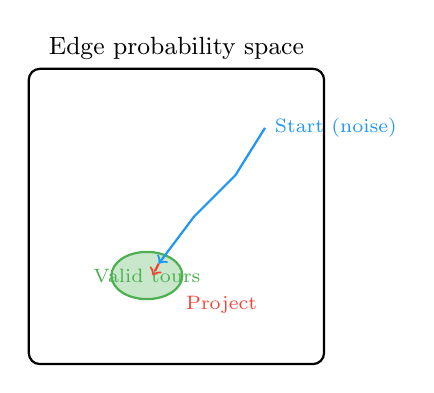
\begin{tikzpicture}[scale=0.75]
    % Large box = edge space
    \draw[thick, rounded corners] (0,0) rectangle (5,5);
    \node[above] at (2.5,5) {\small Edge probability space};

    % Tiny region = valid tours
    \fill[feasgreen, opacity=0.3] (2,1.5) ellipse (0.6 and 0.4);
    \draw[feasgreen, thick] (2,1.5) ellipse (0.6 and 0.4);
    \node[feasgreen, font=\scriptsize] at (2,1.5) {Valid tours};

    % Diffusion path (mostly outside)
    \draw[edisco, thick, ->] (4,4) -- (3.5,3.2) -- (2.8,2.5) -- (2.2,1.7);
    \node[edisco, font=\scriptsize, right] at (4,4) {Start (noise)};

    % Projection arrow
    \draw[warnred, thick, ->, dashed] (2.2,1.7) -- (2.1,1.5);
    \node[warnred, font=\scriptsize, right] at (2.5,1.0) {Project};
\end{tikzpicture}
\end{column}
\end{columns}

\end{frame}

% ============================================================
\begin{frame}{Our Idea: Diffuse on the Feasibility Manifold}

\begin{columns}[T]
\begin{column}{0.55\textwidth}
\textbf{Key insight:} Define diffusion \textbf{directly on the set of valid solutions}, using \textbf{structure-preserving local moves} as transitions.

\vspace{0.5em}
For TSP with 2-opt:
\begin{itemize}
    \item \textbf{State space:} all valid Hamiltonian cycles
    \item \textbf{Transitions:} 2-opt swaps (always produce a valid tour)
    \item \textbf{Forward:} random 2-opt swaps scramble a good tour
    \item \textbf{Reverse:} learned model predicts which swap to apply
\end{itemize}

\vspace{0.5em}
\textcolor{feasgreen}{\textbf{Every state at every timestep is a feasible solution.}}

No decoding. No projection. No repair.
\end{column}
\begin{column}{0.42\textwidth}
\centering
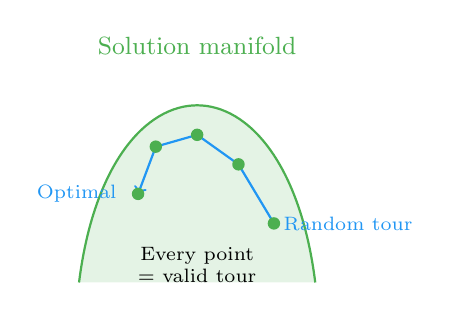
\begin{tikzpicture}[scale=0.75]
    % Manifold shape
    \fill[feasgreen, opacity=0.15] (0.5,0.5) .. controls (1,4.5) and (4,4.5) .. (4.5,0.5) -- cycle;
    \draw[feasgreen, thick] (0.5,0.5) .. controls (1,4.5) and (4,4.5) .. (4.5,0.5);
    \node[feasgreen, font=\small, above] at (2.5,4.2) {Solution manifold};

    % Path on manifold
    \draw[edisco, thick, ->] (3.8,1.5) -- (3.2,2.5) -- (2.5,3.0) -- (1.8,2.8) -- (1.5,2.0);

    % Labels
    \node[edisco, font=\scriptsize, right] at (3.8,1.5) {Random tour};
    \node[edisco, font=\scriptsize, left] at (1.3,2.0) {Optimal};

    % All points on manifold
    \foreach \x/\y in {3.8/1.5, 3.2/2.5, 2.5/3.0, 1.8/2.8, 1.5/2.0} {
        \fill[feasgreen] (\x,\y) circle (3pt);
    }

    \node[font=\scriptsize, text width=3cm, align=center] at (2.5,0.8) {Every point = valid tour};
\end{tikzpicture}
\end{column}
\end{columns}

\end{frame}

% ============================================================
\begin{frame}{Method Overview}

\begin{center}
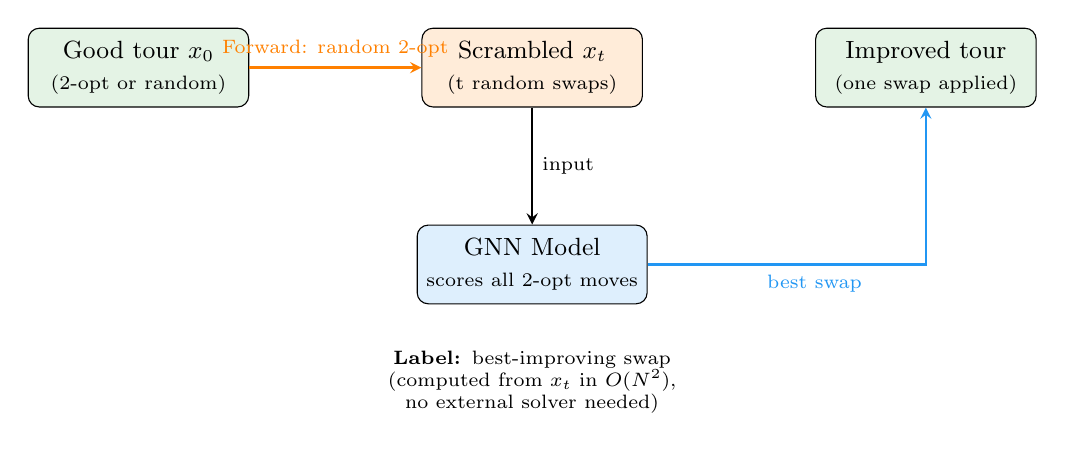
\begin{tikzpicture}[
    box/.style={draw, rounded corners, minimum width=2.8cm, minimum height=1cm, align=center, font=\small},
    arr/.style={->, thick, >=stealth}
]
    % Boxes
    \node[box, fill=feasgreen!15] (x0) at (0,0) {Good tour $x_0$\\{\scriptsize (2-opt or random)}};
    \node[box, fill=orange!15] (xt) at (5,0) {Scrambled $x_t$\\{\scriptsize (t random swaps)}};
    \node[box, fill=edisco!15] (model) at (5,-2.5) {GNN Model\\{\scriptsize scores all 2-opt moves}};
    \node[box, fill=feasgreen!15] (out) at (10,0) {Improved tour\\{\scriptsize (one swap applied)}};

    % Arrows
    \draw[arr, orange] (x0) -- node[above, font=\scriptsize] {Forward: random 2-opt} (xt);
    \draw[arr] (xt) -- node[right, font=\scriptsize] {input} (model);
    \draw[arr, edisco] (model) -| node[below, font=\scriptsize, pos=0.3] {best swap} (out);

    % Training label
    \node[font=\scriptsize, text width=4cm, align=center] at (5,-4) {
        \textbf{Label:} best-improving swap\\
        (computed from $x_t$ in $O(N^2)$,\\
        no external solver needed)
    };
\end{tikzpicture}
\end{center}

\vspace{0.3em}
\textbf{Training:} Cross-entropy on swap prediction. \quad
\textbf{Inference:} Greedy apply predicted swap for $T$ steps.

\textbf{Label-free:} Training data generated entirely by greedy 2-opt trajectories from random starts.

\end{frame}

% ============================================================
\begin{frame}{Key Differences from EDISCO}

\begin{table}[h]
\centering
\renewcommand{\arraystretch}{1.3}
\begin{tabular}{@{}lcc@{}}
\toprule
& \textbf{EDISCO} & \textbf{This Work} \\
\midrule
State during generation & Edge probs $\in [0,1]^{N^2}$ & \textcolor{feasgreen}{\textbf{Valid Hamiltonian cycle}} \\
Intermediate states feasible? & \textcolor{warnred}{No} & \textcolor{feasgreen}{\textbf{Yes, always}} \\
Needs post-hoc decoding? & \textcolor{warnred}{Yes} (greedy + 2-opt) & \textcolor{feasgreen}{\textbf{No}} \\
Search space & Continuous $\mathbb{R}^{N^2}$ & Discrete valid tours \\
External solver for labels? & \textcolor{warnred}{Yes} (Concorde) & \textcolor{feasgreen}{\textbf{No}} (self-generated) \\
Equivariant? & Yes (E(2)) & Yes (E(2)-compatible) \\
\bottomrule
\end{tabular}
\end{table}

\vspace{0.5em}
\textbf{Same mathematical framework} (CTMC), \textbf{different state space} (valid solutions, not edge probabilities).

\end{frame}

% ============================================================
\begin{frame}{Preliminary Results: TSP-50}

\begin{columns}[T]
\begin{column}{0.48\textwidth}
\textbf{Setup:} TSP-50, 5000 self-generated instances, \textbf{no optimal labels}, GNN 6-layer 128-dim (694K params).

\vspace{0.5em}
\textbf{Results (vs 2-opt reference):}
\begin{itemize}
    \item Best gap: \textbf{$-$0.01\%} (matches 2-opt)
    \item Cost: 27.0 $\to$ 5.97 in 150 steps
    \item All intermediate tours: \textcolor{feasgreen}{\textbf{FEASIBLE}}
\end{itemize}

\vspace{0.5em}
{\small \textit{Gap to true optimal (OR-Tools) $\approx$ 3--5\%.\\Closable with optimal labels.}}
\end{column}
\begin{column}{0.50\textwidth}
\centering
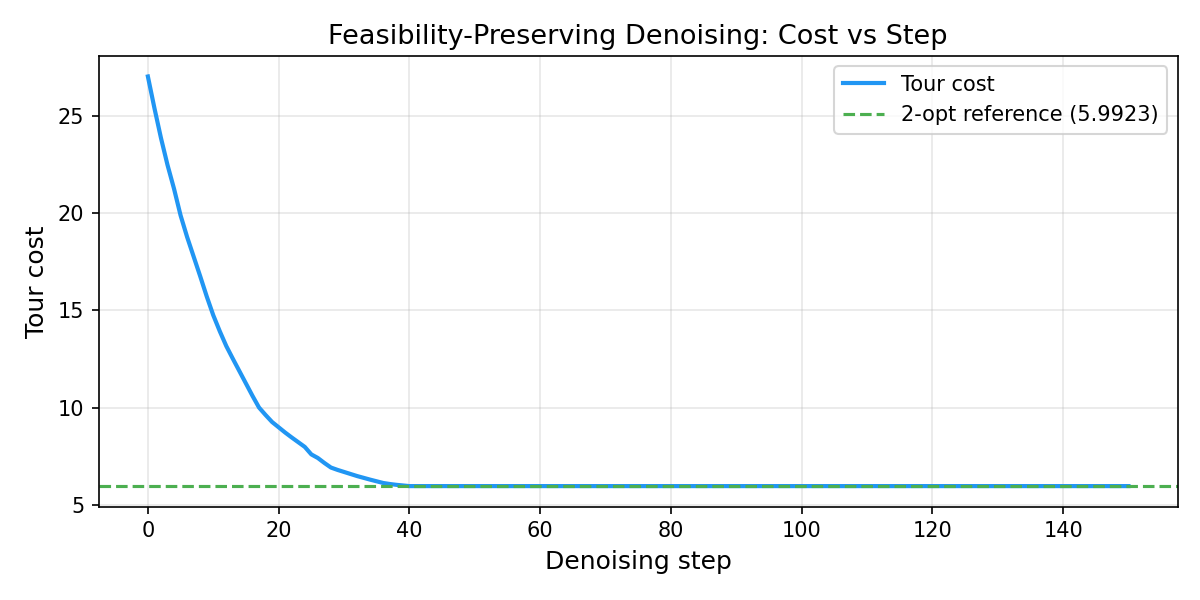
\includegraphics[width=\textwidth]{../denoise_tsp50_inst0_cost.png}

\vspace{0.2em}
{\small Cost decreases monotonically.\\Every point on the curve is a valid tour.}
\end{column}
\end{columns}

\end{frame}

% ============================================================
\begin{frame}{Visualization: Denoising on the Feasibility Manifold}

\begin{columns}[c]
\begin{column}{0.32\textwidth}
\centering
\textbf{Step 0} (Random)\\[0.3em]
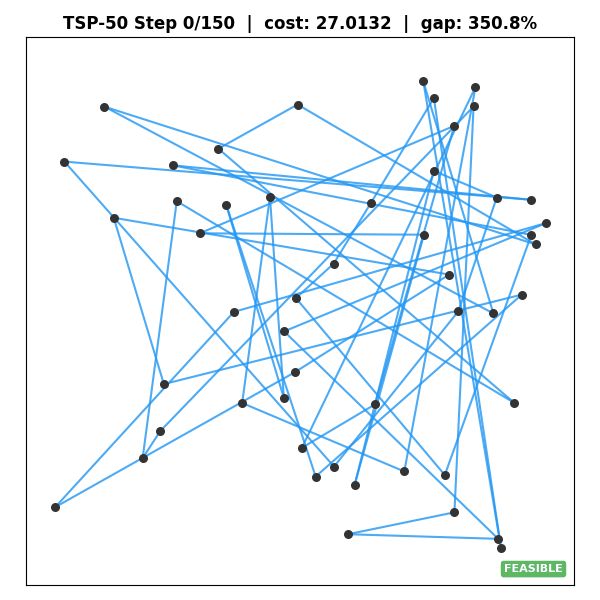
\includegraphics[width=\textwidth]{../frame_start.png}
{\small Cost = 27.0\\Gap = 351\%}
\end{column}
\begin{column}{0.32\textwidth}
\centering
\textbf{Step 35} (Improving)\\[0.3em]
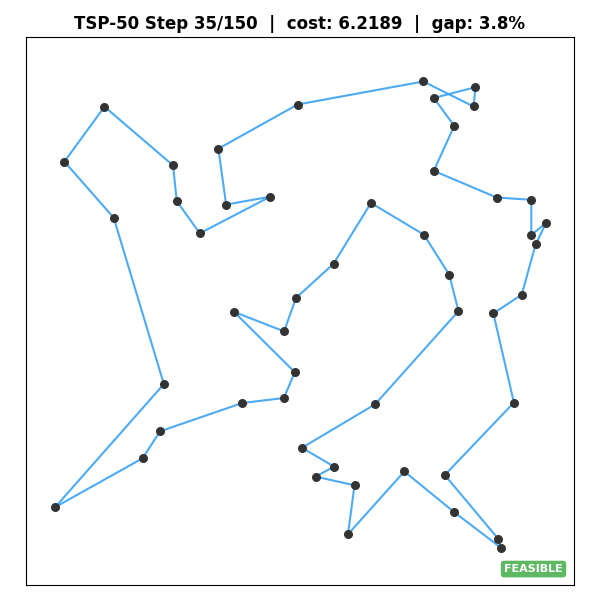
\includegraphics[width=\textwidth]{../frame_mid.png}
{\small Cost = 6.22\\Gap = 3.8\%}
\end{column}
\begin{column}{0.32\textwidth}
\centering
\textbf{Step 70} (Converged)\\[0.3em]
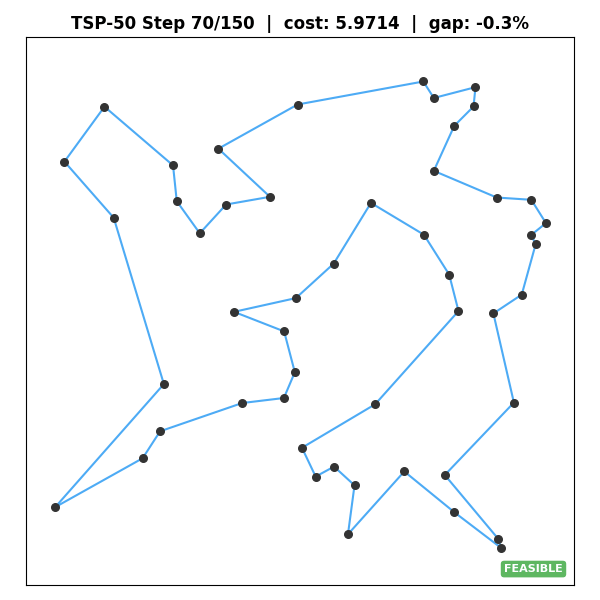
\includegraphics[width=\textwidth]{../frame_end.png}
{\small Cost = 5.97\\Gap = $-$0.3\%}
\end{column}
\end{columns}

\vspace{0.8em}
\centering
\textcolor{feasgreen}{\textbf{Every frame is a valid Hamiltonian cycle.}} {\small (See GIF for full animation.)}

\end{frame}

% ============================================================
\begin{frame}{Novelty and Next Steps}

\textbf{Confirmed novel} (exhaustive literature survey, April 2026):
\begin{itemize}
    \item No prior work defines diffusion on the \textbf{feasibility manifold} with local-search transitions
    \item Closest: Neural Simulated Annealing (AISTATS'23) --- learned MCMC, not diffusion
\end{itemize}

\vspace{0.5em}
\textbf{Immediate next steps:}
\begin{enumerate}
    \item Use \textbf{optimal labels} (OR-Tools) to push beyond 2-opt ceiling
    \item Add \textbf{E(2)-equivariant GNN} (from EDISCO) as the backbone
    \item \textbf{Scale test:} train on TSP-50, evaluate on TSP-500/1000 (equivariance $\to$ generalization)
    \item Extend to \textbf{CVRP} (swap transitions on feasible partitions)
\end{enumerate}

\vspace{0.5em}
\textbf{Target venue:} NeurIPS 2026 or ICLR 2027

\end{frame}

\end{document}
